
%提出するレポートの書式はこのtemplateファイルに沿って作成してください。
%特に表紙・概要の書式は変えないで下さい。

\documentclass[a4j]{jarticle}

\usepackage[dvipdfmx]{graphicx}
%\usepackage{epsbox}
\usepackage{url}
\usepackage{here}
\usepackage{amsmath,amssymb}
\setlength{\headsep}{-5mm}
\setlength{\oddsidemargin}{0mm}
\setlength{\textwidth}{165mm}
\setlength{\textheight}{230mm}
\setlength{\footskip}{20mm}

\title{
\vspace{30mm}
{\bf 高知工科大学様}
\\
\vspace{5mm}
大学掲示板(KUTBBS)\\
\vspace{5mm}
{\bf  外部設計書v0.1}
\vspace{90mm}
}

\author{
\vspace{5mm}
グループ10 \\
\vspace{5mm}
Pathfinder \\
\vspace{5mm}
\vspace{10mm}
}

%date{
%平成30年8月1日
%}

\begin{document}
\maketitle
\tableofcontents
\newpage




\section{システムの利用と業務の流れ}
本システムは、学生が陥りやすいトラブルや、学生自身の学習における課題や悩みを自主的に解決するための掲示板型のウェブアプリケーションである。近年の情報収集におけるツールと言えば、専らスマートフォンを用いた情報検索であるが、それが必ずしも問題を解決するとは限らない。そこで、(本校の)学生同士が問題をネット上でかつ匿名に解決できるようにするために開発するシステムが、本システムである。



本システムを利用する対象は、本校の学生である。また管理者は、本校の事務員を想定している。新規利用者は、まず事前に配布される仮ID・パスワードを受け取りこれを本システムに入力することで、ログインすることができる。仮ID・パスワードをそのまま使い続けるのはセキュリティ上好ましくないため、初回ログイン後速やかに変更を促す。管理者の登録については親管理者のみが行える仕様になっている(詳細な仕様はサブシステムの項目で述べる)。登録された管理者は、管理するための業務を行えるようになる。


登録を終えた利用者は、本システムを利用することが可能になる。利用者は、以下のような主な掲示板の機能を利用することができる。
\begin{itemize}
  \item スレッドの作成及び閲覧
  \item スレッドへの書き込み
  \item ブックマーク機能
  \item スレッド検索
  \item 良いレスに対してアクションを返す機能
  \item 不適切なレスやスレッドの通報
\end{itemize}



管理者が行う主な業務としては、仮ID・パスワード発行と、前述したような例にあたる不適切なスレッドやレスの削除である。また、不適切なスレッドやレスを繰り返し行う悪質なユーザに対して警告や、懲罰措置を行うことも想定されている。そのため、管理者は以下のような機能を利用することができる。
なお親管理者については、これらの操作に加えて管理者の登録も可能である。

\begin{itemize}
  \item 仮ID・及びパスワードの発行
  \item スレッドやレスの削除
  \item 通報されてきたスレッドやレスの閲覧
  \item ユーザの情報閲覧
  \item 不適切なユーザへの警告・懲罰機能
  \item 管理者の登録(親管理者のみ)
\end{itemize}





以下に本システムの利用の一例とその過程を示しながら、管理者の業務の流れを示す。

\begin{enumerate}
  \item 利用者Aは自身が興味のあるスレッドを閲覧し、書き込みを行った。スレッドを閲覧するために必要な情報は、対象のスレッドに書き込まれたレスの情報のみである。書き込みの際に必要となる情報は、自身の書き込み内容である。

  \item  利用者が書き込みを行った後、再度書き込みを行ったスレッドを閲覧すると、自分の書き込み宛に誹謗中傷をする書き込みがあったため、管理者に通報を行った。通報を行う際に必要な情報は、不適切なレスが行われたスレッドタイトルと書き込み内容、それに通報の理由である。
  \item  管理者は、Webブラウザから管理者ページにログインし、利用者から通報されてきたレス及びスレッドを確認するページを閲覧する。管理者は、そのページを閲覧し、公序良俗に著しく欠けるタイトルやレスに対して、削除を行った。
\end{enumerate}

図1は上記の流れを表したものである。


\begin{figure}[h!]
\begin{center}
\resizebox{10cm}{!}{\includegraphics{flow.png}}
\caption{上記の業務の流れ}
\label{fig:figuretest}
\end{center}
\end{figure}














\section{システム概要}
本システムは機能として下記に示す「ユーザ機能」、「掲示板機能」、「管理者機能」の3つを実装する。
 また、各機能を構成するサブシステムも併せて示す。それぞれのサブシステムに関しては3章にて詳細を述べる。

\subsection{ユーザ機能}
 ユーザ機能では、ユーザのアカウント登録や、本システムへのログインをすることができる。また、各ユーザが各種設定を変更したり、お知らせを閲覧したり、ブックマークしたスレッドを容易に閲覧することができる。
\\【構築サブシステム】
\\ ブックマークサブシステム、マイページサブシステム、アカウント登録サブシステム
\\ ログインサブシステム、お知らせ表示サブシステム

\subsection{掲示板機能}
 掲示板機能では、大学の在学生同士の情報共有の場を提供する。見たいスレッドを検索することができ、
 自分が作成したスレッドに対するレスがついたことを通知できる。また、不適切なスレッドまたはレスに対しては管理者に通報ができる。
 信頼性があるレスに対しては、コレクトボタンを押し、情報の信頼性を示すことができる。
\\【構築サブシステム】
\\ 検索サブシステム、掲示板サブシステム
\\ 通報サブシステム、通知サブシステム、コレクトボタンサブシステム

\subsection{管理者機能}
 管理者機能では、本システムを管理するための管理者のみが使用できるシステムが備わっている。
\\【構築サブシステム】
\\ 子管理者管理サブシステム、お知らせ編集サブシステム、掲示板編集サブシステム
\\ 利用者管理サブシステム、利用者登録サブシステム、管理者ログインサブシステム

\section{サブシステム設計}
2章で述べた3つの機能を構成するサブシステムの概要と詳細について利用者側、管理者側に分けて述べる。

\subsection{サブシステム概要(利用者)}
本システムのサブシステムには、下記のサブシステムが存在する。
\begin{enumerate}
\item アカウント登録サブシステム\\
大学から与えられた仮IDと仮パスワードから利用者専用のIDとパスワードへ変更し、アカウント登録を行う。

\item ログインサブシステム\\
利用者が設定したIDとパスワードを入力することで自分のアカウントへのログインを行う。

\item お知らせ表示サブシステム\\
管理者からのお知らせを閲覧することができる。

\item 検索サブシステム\\
過去に作成されたスレッドの検索を行うことができる。


\item 掲示板サブシステム\\
利用者がスレッドの作成・レスの書き込みを行うことができる。


\item 通報サブシステム\\
利用者が、誹謗中傷や公序良俗に違反していると考えられるスレッドまたはレスを管理者に通知させることができる。


\item ブックマークサブシステム\\
利用者は頻繁に訪問するスレッドを登録することができる。


\item 通知サブシステム\\
利用者が作成したスレッドに対して、レスが書き込まれた場合、または利用者が書き込んだレスに対して返信が書き込まれた場合に、利用者に通知を送ることができる。


\item コレクトボタンサブシステム\\
利用者が投稿したレスに対して、投稿した本人以外の利用者がその投稿内容が確からしいと判断したときに、コレクトボタンを押し、コレクト認定をする。コレクト認定された回数が多いほど、そのレスは信頼性が高いと判断できる。


\item マイページサブシステム\\
マイページでは、利用者が各種設定を行うことができる。また、利用者に対する通知がマイページに表示される。
\end{enumerate}

\subsection{サブシステム詳細(利用者)}
各サブシステムの詳細を以下に示す。
\begin{enumerate}
  \item アカウント登録サブシステム\\
  アカウント登録サブシステムは以下の機能によって構成される。
  \begin{itemize}
    \item 新規登録機能\\
    新規登録時、ID・パスワード入力画面に遷移する。利用者は大学から配布された仮IDと仮パスワードを入力することで、ID・パスワード変更画面に遷移することができる。その後、利用者は各自でIDとパスワードを変更し、登録を行うことができる。なお、IDとパスワードを登録しなければ、本システムは利用することができない。
  \end{itemize}

  \item ログインサブシステム\\
  ログインサブシステムは以下の機能によって構成される。
  \begin{itemize}
    \item ユーザ認証機能\\
    本システムを利用する利用者が、本学の在学生であるかの認証を、IDとパスワードを用いて行う。認証に成功した利用者は、本システムの正当な利用者として本システムを利用することができる。
    \item ログインボーナス機能\\
    利用者が本システムにログインしたとき、拡張機能と交換できるポイントが付与される。ポイントが付与される頻度は、1日1回である。1回で付与されるポイント数は10ポイントである。
    \item ログアウト機能\\
    利用者が本システムにログインしている状態であるとき、「ログアウト」のボタンをタップすることで本システムからログアウトすることができる。
  \end{itemize}

  \item お知らせ表示サブシステム\\
  お知らせサブシステムは以下の機能によって構成される。
  \begin{itemize}
    \item お知らせ閲覧機能\\
    管理者から通達されたお知らせを閲覧することができる。
  \end{itemize}

  \item 検索サブシステム\\
  検索サブシステムは以下の機能によって構成される。
  \begin{itemize}
    \item 検索機能\\
    所定の検索窓に任意の文字列を入力し、その文字列に関連したスレッドを一覧で表示することができる。検索方法はand検索、or検索が使用可能である。
    \item カテゴリ選択機能\\
    所定の検索窓の横に設置されたカテゴリ選択ボタンで特定のカテゴリを選択すると、選択されたカテゴリ内に存在するスレッドの中から検索することができる。
  \end{itemize}

  \item 掲示板サブシステム\\
  掲示板サブシステムは以下の機能によって構成される。
  \begin{itemize}
    \item スレッド作成機能\\
    スレッドタイトルとそのスレッドの説明を付与して、新規のスレッドを作成することができる。
    \item レス書き込み機能\\
    既存のスレッド内に、レスを書き込むことができる。このとき、レス番号・ハンドルネーム・日付・レスIDが表示される。レスの書き込み主がハンドルネームを設定している場合、そのハンドルネームが表示される。
  \end{itemize}

  \item 通報サブシステム\\
  通報サブシステムは以下の機能によって構成される。
  \begin{itemize}
    \item スレッド・レス通報機能\\
    利用者が誹謗中傷や公序良俗に違反するなどの不適切な内容であると判断したスレッドまたはレスを管理者に通報することができる。このとき、通報者は通報理由を明記しなければならない。
  \end{itemize}

  \item ブックマークサブシステム\\
  ブックマークサブシステムは以下の機能によって構成される。
  \begin{itemize}
    \item ブックマーク登録機能\\
    任意のスレッドをブックマークとしてマイページに登録することができる。
    \item ブックマーク解除機能\\
    マイページに存在する任意のブックマークの登録を解除することができる。
  \end{itemize}

  \item 通知サブシステム\\
  通知サブシステムは以下の機能によって構成される。
  \begin{itemize}
    \item 通知機能\\
    利用者が作成したスレッドに新たな書き込みがあった場合、または利用者が書き込んだレスに対して返信が書き込まれた場合に、その旨をマイページに通知する。
  \end{itemize}

  \item コレクトボタンサブシステム\\
  コレクトボタンサブシステムは以下の機能によって構成される。
  \begin{itemize}
    \item コレクト認定機能\\
    利用者が特定のレスに対して、その内容が確からしいと判断した場合、コレクトボタンを押してコレクト認定をすることができる。レスの傍らにコレクト認定された回数が表示されるため、コレクト認定は、利用者がそのレスの内容が確からしいと判断した指標となる。よって、コレクト認定された回数が多いレスは、信憑性のある情報として、利用者の情報の取捨選択の判断材料となる。なお、1つのレスに対してコレクト認定できる回数は1回のみであり、コレクトボタンを偶数回押すと、コレクト認定を解除することができる。
    \item ポイント獲得機能\\
    利用者が書き込んだレスに他の利用者からコレクト認定された場合、レスの書き込み主に拡張機能を解放するためのポイントを獲得することができる。
  拡張機能とは、スレッドでレスを行う際にレスの表示が変化する機能である。
    ポイント獲得の相場は、1回のコレクト認定につき1ポイントである。1つのレスにおいて、1人のユーザからポイント獲得できる回数は1回のみである(2回目以降のコレクト認定はポイント獲得できない)。また、コレクト認定が解除されたとしても獲得済のポイントが減ることはない。
  \end{itemize}

  \item マイページサブシステム\\
  マイページサブシステムは以下の機能によって構成される。
  \begin{itemize}
    \item ユーザ情報設定機能\\
    利用者のハンドルネームの設定ができる。ハンドルネームが設定されていない場合は、「名無し」と表示される。
    \item ブックマーク閲覧機能\\
    登録したブックマークの一覧を表示することができる。その中から、任意のスレッドに遷移することができる。
    \item 拡張機能\\
    本システムを利用して得られたポイントと引き換えに、拡張機能が使用可能となる。主な拡張機能としては、取り消し線、太文字、赤字、斜体などが存在する。1つの拡張機能につき、600ポイントを引き換えると想定する。拡張機能は、今後の仕様変更で追加する可能性がある。
    \item 通知設定機能\\
    通知機能のON/OFFの設定をすることができる。
  \end{itemize}
\end{enumerate}



\subsection{サブシステム概要(管理者)}
 管理者ページのサブシステムには下記のサブシステムが存在する。
\begin{enumerate}
  \item 子管理者管理サブシステム\\
  親管理者が子管理者のアカウントを管理するシステムである。親管理者がIDとパスワードを発行することで、本システムを管理する子管理者を登録する。また、不要になった子管理者のアカウントを抹消する。


  \item お知らせ編集サブシステム\\
  管理者から利用者全体に対して任意のお知らせを通達することができる。


  \item 掲示板編集サブシステム\\
  管理者は不適切であると判断したスレッドやレスを削除または置換することができる。


  \item 利用者管理サブシステム\\
  管理者は利用者の情報を検索し、閲覧することができる。また、不適切なスレッドやレスを書き込んだ利用者に対して警告やアカウント凍結などの処置を行うことができる。


  \item 利用者登録サブシステム\\
  管理者は利用者の仮IDと仮パスワードの発行を行うことができる。仮IDと仮パスワードを用いて、利用者は本システムに新規登録することができる。


  \item 管理者ログインサブシステム\\
  管理者は学内LANに接続された電子デバイスからのみ、管理者のIDとパスワードを入力することで、管理者として本システムにログインすることができる。
\end{enumerate}

\subsection{サブシステム詳細(管理者)}
各サブシステムの詳細を以下に示す。
\begin{enumerate}

  \item 子管理者管理サブシステム\\
  子管理者管理サブシステムは以下の機能によって構成される。
  \begin{itemize}
    \item 子管理者用ID・パスワード発行機能\\
    親管理者は手動で子管理者用のIDとパスワードを登録し、発行することができる。ただし、子管理者にはこの機能は存在しない。
    \item 子管理者アカウント抹消機能\\
    親管理者は手動で不要になった子管理者のアカウントを抹消することができる。
    \item 子管理者情報閲覧機能\\
    親管理者は子管理者のIDとパスワードを閲覧することができる。
  \end{itemize}


  \item お知らせ編集サブシステム\\
  お知らせ編集サブシステムは以下の機能によって構成される。
  \begin{itemize}
    \item お知らせ編集機能\\
    管理者は、利用者に対して通達するお知らせタイトルとその内容を編集することができる。
    \item お知らせ表示機能\\
    本システムのトップページに、上記で編集したお知らせの日付とお知らせタイトルを表示することができる。
    \item お知らせリンク機能\\
    上記で編集したお知らせ内容を本システムトップページに表示されているお知らせタイトルにリンクを追加することができる。\\
  \end{itemize}


  \item 掲示板編集サブシステム\\
   掲示板編集サブシステムは以下の機能によって構成される。
  \begin{itemize}
    \item スレッド削除機能\\
    管理者は、データベースに存在するスレッド及びスレッドに格納された全てのレスを削除することができる。ただし、このときのスレッドは完全に削除されるわけではなく、削除履歴として別のテーブルに保存される。
    \item レス削除機能\\
    管理者は、データベースに存在するスレッド内のレスを削除することができる。ただし、このときのレスは完全に削除されるわけではなく、削除履歴として別のテーブルに保存される。
    \item 削除履歴閲覧機能\\
    管理者は、削除したスレッドまたはレスを一覧で閲覧することができる。
    \item 不適切な単語登録機能\\
    管理者は、誹謗中傷や公序良俗に違反していると考えられる単語を登録することができる。
    \item 不適切な単語自動置換機能\\
    管理者が設定した不適切な単語を検出し次第、自動で伏せ字に置換することができる。
    \item 通報内容閲覧機能\\
    利用者によって通報されたスレッドまたはレスの内容の一覧を、通報理由と共に閲覧することができる。このとき、通報者のユーザ情報、通報されたスレッド主またはレスの書き込み主のユーザ情報も同時に表示される。\\
  \end{itemize}


  \item 利用者管理サブシステム\\
   利用者管理サブシステムは以下の機能によって構成される。
  \begin{itemize}
    \item 利用者情報閲覧機能\\
    管理者は、データベースに登録されている任意の利用者情報を閲覧することができる。
    \item 利用者情報検索機能\\
    管理者は、データベースに登録されている利用者情報の中から特定の利用者情報を検索することができる。
    \item 利用者に対する警告通知送信機能\\
    管理者は、不適切な内容のスレッド作成またはレスの書き込みを度々行った利用者に対して、注意喚起の旨を利用者のマイページに通知することができる。
    \item 利用者アカウント凍結機能\\
    管理者は、度重なる注意を通達したにも関わらず、迷惑行為が改善されない利用者のアカウントに対して、書き込み不可能にすることができる。\\
  \end{itemize}


  \item 利用者登録サブシステム\\
   利用者登録サブシステムは以下の機能によって構成される。
  \begin{itemize}
    \item 仮ID・仮パスワード発行機能\\
    管理者は仮IDと仮パスワードを発行することができる。仮IDと仮パスワードの生成には、乱数を用いる。\\
  \end{itemize}


  \item 管理者ログインサブシステム\\
   管理者ログインサブシステムは以下の機能によって構成される。
  \begin{itemize}
    \item 管理者認証機能\\
    本システムの管理作業を行う利用者が、管理者であるかの認証を、IDとパスワードを用いて行う。認証に成功した利用者は管理者として本システムの管理を行うことができる。
  \end{itemize}

\end{enumerate}



\section{ユーザインタフェース設計}

\subsection{画面遷移図}


\section{データベース設計}
本システムに用いるデータについて以下に示す。
\subsection{データテーブル仕様}
本システムのデータベースには、9個のデータテーブルが存在する。各データテーブルの仕様をデータモデルを用いて以下に示す。
\begin{itemize}
\item ユーザテーブル\\
  ユーザテーブルでは本システムを利用するユーザに関する情報を管理する。またフラグを用いることで利用者と管理者(親管理者と子管理者)を区別、拡張機能の寄与、初回ログインの判別を行っている。表1にこのテーブルのデータモデルを示す。
  \begin{table}[h]
    \caption{ユーザモデル}
    \begin{center}
      \begin{tabular}{|l|c|l|} \hline

        \multicolumn{1}{|c|}{属性} & データ型 & \begin{tabular}{c}キー:テーブル名\end{tabular}\\\hline \hline
          学生番号&CHAR(10)&PK\\\hline
          ユーザID&CHAR(20)&  \multicolumn{1}{|c|}{-} \\\hline
          パスワード&CHAR(20)& \multicolumn{1}{|c|}{-}\\\hline
          保有ポイント&INT& \multicolumn{1}{|c|}{-}\\\hline
          拡張機能フラグ1(VIPフラグ)&CHAR(1)& \multicolumn{1}{|c|}{-}\\\hline
          拡張機能フラグ2(色)&CHAR(2)& \multicolumn{1}{|c|}{-}\\\hline
          拡張機能フラグ3(太字)&CHAR(1)& \multicolumn{1}{|c|}{-}\\\hline
          拡張機能フラグ4(斜線)&CHAR(1)& \multicolumn{1}{|c|}{-}\\\hline
          初回ログインフラグ&CHAR(1)& \multicolumn{1}{|c|}{-}\\\hline
          管理者フラグ&CHAR(1)& \multicolumn{1}{|c|}{-}\\\hline
      \end{tabular}
    \end{center}
  \end{table}
\item スレッドテーブル\\
  スレッドテーブルではスレッドに関する情報を管理する。表2にこのテーブルのデータモデルを示す。

  \begin{table}[h]
    \caption{スレッドモデル}
    \begin{center}
      \begin{tabular}{|l|c|c|} \hline

        \multicolumn{1}{|c|}{属性} & データ型 & \begin{tabular}{c}キー:テーブル名\end{tabular}\\\hline \hline
          スレッドID&CHAR(10)&\multicolumn{1}{|l|}{PK}\\\hline
          スレッドカテゴリID&CHAR(2)&\multicolumn{1}{|l|}{FK:スレッドカテゴリテーブル}\\\hline
          スレッドタイトル&CHAR(50)& -\\\hline
          作成日時&DATE()& -\\\hline
          更新日時&DATE()& -\\\hline
      \end{tabular}
    \end{center}
  \end{table}
  \newpage
\item お気に入り掲示板テーブル\\
  お気に入り掲示板テーブルではユーザが気に入ったスレッドに対してブックマークとして登録したスレッド情報を管理する。表3にこのテーブルのデータモデルを示す。

  \begin{table}[h]
    \caption{お気に入り掲示板モデル}
    \begin{center}
      \begin{tabular}{|l|c|c|} \hline
        \multicolumn{1}{|c|}{属性} & データ型 & \begin{tabular}{c}キー:テーブル名\end{tabular}\\\hline \hline
          学籍番号&CHAR(10)&\multicolumn{1}{|l|}{FK:ユーザテーブル}\\\hline
          スレッドID&CHAR(10)&\multicolumn{1}{|l|}{FK:スレッドテーブル}\\\hline
      \end{tabular}
    \end{center}
  \end{table}

\item レステーブル\\
  レステーブルではスレッドに対してのレスに関する情報を管理する。表4にこのテーブルのデータモデルを示す。
  \begin{table}[h]
    \caption{レスモデル}
    \begin{center}
      \begin{tabular}{|l|c|c|} \hline
        \multicolumn{1}{|c|}{属性} & データ型 & \begin{tabular}{c}キー:テーブル名\end{tabular}\\\hline \hline
          レスID&CHAR(10)&\multicolumn{1}{|l|}{PK(スレッドIDと複合)}\\\hline
          スレッドID&CHAR(10)&\multicolumn{1}{|l|}{PK(レスIDと複合)、FK:スレッドテーブル}\\\hline
          学籍番号&CHAR(10)&\multicolumn{1}{|l|}{FK:ユーザテーブル}\\\hline
          書き込みID&N VCHAR(15)&-\\\hline
          書き込み内容&N VCHAR(200)&-\\\hline
          コレクトボタンプッシュ数&INT&-\\\hline
          レス日時&-&-\\\hline
      \end{tabular}
    \end{center}
  \end{table}

\item コレクトユーザテーブル\\
  コレクトユーザテーブルでは利用者が投稿したレスに対して、投稿した本人以外の利用者がそのレスに対して信頼性があると判断した場合に、コレクトボタンを押されたことに関する情報を管理する。表5にこのテーブルのデータモデルを示す。
  \begin{table}[h]
    \caption{コレクトユーザモデル}
    \begin{center}
      \begin{tabular}{|l|c|c|} \hline
        \multicolumn{1}{|c|}{属性} & データ型 & \begin{tabular}{c}キー:テーブル名\end{tabular}\\\hline \hline
          学籍番号&CHAR(20)&\multicolumn{1}{|l|}{FK:ユーザテーブル}\\\hline
          スレッドID&CHAR(10)&\multicolumn{1}{|l|}{FK:スレッドテーブル}\\\hline
          レスID&CHAR(10)&\multicolumn{1}{|l|}{FK:レステーブル}\\\hline
      \end{tabular}
    \end{center}
  \end{table}
  \newpage
\item NGワードテーブル\\
  NGワードテーブルでは管理者が誹謗中傷や公序良俗に違反していると考えられる単語を登録したNGワードの情報を管理する。表6にこのテーブルのデータモデルを示す。
  \begin{table}[h]
    \caption{NGワードモデル}
    \begin{center}
      \begin{tabular}{|l|c|c|} \hline
        \multicolumn{1}{|c|}{属性} & データ型 & \begin{tabular}{c}キー:テーブル名\end{tabular}\\\hline \hline
          NGワードID&CHAR(5)&\multicolumn{1}{|l|}{PK}\\\hline
          NGワード&N VCHAR(20)&-\\\hline
      \end{tabular}
    \end{center}
  \end{table}
\item スレッドカテゴリテーブル\\
  スレッドカテゴリテーブルでは各カテゴリごとに分けられたスレッドの情報を管理する。表7にこのテーブルのデータモデルを示す。
  \begin{table}[h]
    \caption{スレッドカテゴリモデル}
    \begin{center}
      \begin{tabular}{|l|c|c|} \hline
        \multicolumn{1}{|c|}{属性} & データ型 & \begin{tabular}{c}キー:テーブル名\end{tabular}\\\hline \hline
          カテゴリID&CHAR(2)&\multicolumn{1}{|l|}{PK}\\\hline
          カテゴリ名&N VCHAR(15)&-\\\hline
      \end{tabular}
    \end{center}
  \end{table}
\item  通報テーブル\\
  通報テーブルでは利用者が謗中傷や公序良俗に違反するなどの不適切な内容であると判断したスレッドまたはレスを管理者に通報した時の情報を管理する。また、通報した内容の情報も管理する。表8にこのテーブルのデータモデルを示す。
  \begin{table}[h]
    \caption{通報モデル}
    \begin{center}
      \begin{tabular}{|l|c|c|} \hline
        \multicolumn{1}{|c|}{属性} & データ型 & \begin{tabular}{c}キー:テーブル名\end{tabular}\\\hline \hline
          通報ID&CHAR(10)&\multicolumn{1}{|l|}{PK}\\\hline
          通報ユーザID&CHAR(10)&\multicolumn{1}{|l|}{FK:ユーザテーブル}\\\hline
          スレッドID&CHAR(10)&\multicolumn{1}{|l|}{FK:スレッドテーブル}\\\hline
          レスID&CHAR(10)&\multicolumn{1}{|l|}{FK:レステーブル}\\\hline
          通報カテゴリID&CHAR(10)&\multicolumn{1}{|l|}{FK:通報カテゴリテーブル}\\\hline
          通報内容&N VCHAR(200)&-\\\hline
          通報日時&DATE()&-\\\hline
      \end{tabular}
    \end{center}
  \end{table}
        \newpage
      \item BANテーブル\\
        BANテーブルでは、迷惑行為が改善されない利用者のアカウントに対しての情報を管理する。表9にこのテーブルのデータモデルを示す。
          \begin{table}[h]
    \caption{ユーザ凍結モデル}
    \begin{center}
      \begin{tabular}{|l|c|c|} \hline
        \multicolumn{1}{|c|}{属性} & データ型 & \begin{tabular}{c}キー:テーブル名\end{tabular}\\\hline \hline
          BANID&CHAR(5)&\multicolumn{1}{|l|}{PK}\\\hline
          学籍番号&CHAR(10)&\multicolumn{1}{|l|}{FK:ユーザテーブル}\\\hline

      \end{tabular}
    \end{center}
  \end{table}

\end{itemize}
\subsection{データテーブルの構造}
本システムのデータテーブルの構造についてはERモデルを用いて図()で示す。

\begin{figure}[h!]
\begin{center}
\resizebox{10cm}{!}{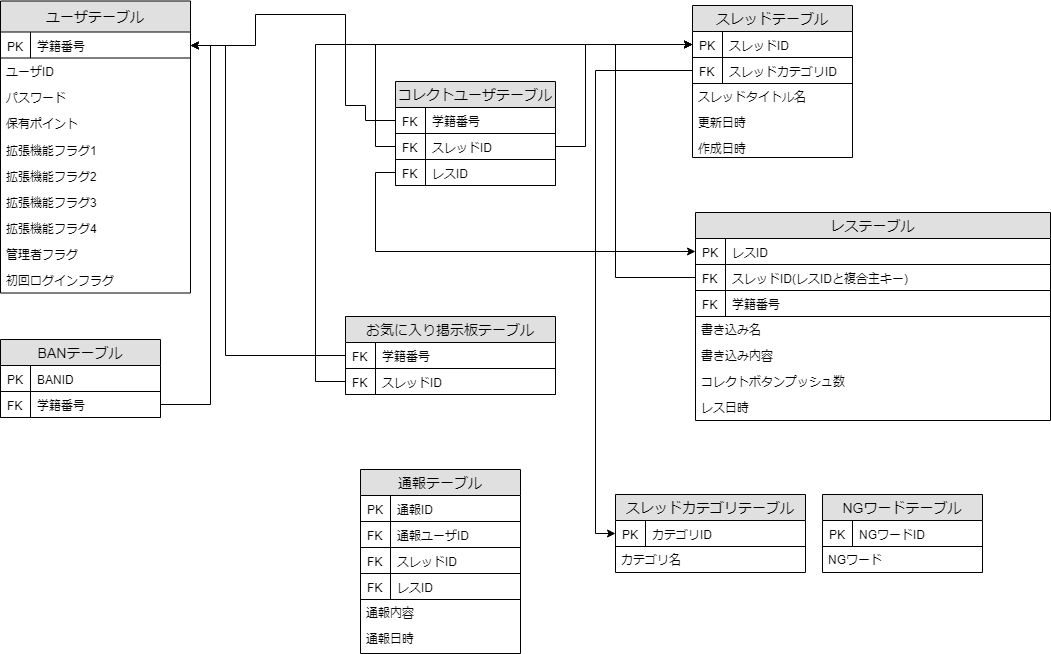
\includegraphics{KUTBBS.png}}
\caption{データベースのER図}
\label{ER:ERtest}
\end{center}
\end{figure}


\section{ネットワーク設計}




% \bibliographystyle{jplain}
% \begin{thebibliography}{10}
%
%
%
% \end{thebibliography}


\end{document}
